\chapter{Espelhos e reflexão}\label{ch:g5:mirrors-reflection}

A \omterm{def:g1:light-and-shadows:source}{luz}, como provamos, nunca faz curva nas esquinas --- e mesmo assim
toda manhã uma cópia de você olha de dentro da parede do banheiro, e
no ano passado prometemos um truque para, apesar de tudo, enxergar
depois de uma esquina. O truque não é entortar a estrada, e sim
\emph{dobrá-la}. Tudo se dobra numa superfície notável: o \omterm{def:g5:mirrors-reflection:reflection}{espelho}.

\section{O quique}

\begin{definition}[Reflexão]\label{def:g5:mirrors-reflection:reflection}
Quando a \omterm{def:g1:light-and-shadows:source}{luz} bate numa superfície e volta em vez de atravessá-la ou
morrer ali, chamamos isso de \emph{reflexão}\index{reflexão}: a \omterm{def:g1:light-and-shadows:source}{luz} é
refletida. Um \emph{espelho}\index{espelho} é uma superfície tão lisa
que reflete a \omterm{def:g1:light-and-shadows:source}{luz} de um jeito perfeitamente ordenado --- metal polido
atrás de um vidro, água parada, uma colher reluzente.
\end{definition}

\begin{proposition}[A regra do quique]\label{prop:g5:mirrors-reflection:bounce}
Um \omterm{def:g4:light-straight-lines:ray}{raio de luz} quica num \omterm{def:g5:mirrors-reflection:reflection}{espelho} do mesmo jeito que uma bola perfeita
quica numa parede: ele sai exatamente com a mesma inclinação com que
chegou, do outro lado. Reto para dentro --- reto de volta. Inclinado
para dentro --- inclinado para fora com a inclinação
correspondente. Os dois ângulos, o de chegada e o de saída, são
sempre iguais.
\end{proposition}

\begin{omfigure}
\begin{tikzpicture}[scale=0.85]
  \draw[very thick] (0.5,0) -- (10.5,0);
  \foreach \x in {1.0,1.75,...,10.0} {
    \draw[thin] (\x,0) -- (\x-0.3,-0.3);
  }
  \draw[-Stealth, very thick, omThm] (2.0,3.0) -- (5.5,0.05);
  \draw[-Stealth, very thick, omThm] (5.5,0.05) -- (9.0,3.0);
  \draw[dashed] (5.5,0) -- (5.5,3.2);
  \draw[omExo, thick] (4.42,0.95) arc (140:90:1.45);
  \draw[omExo, thick] (6.58,0.95) arc (40:90:1.45);
  \node[font=\small] at (4.7,1.75) {chega};
  \node[font=\small] at (6.35,1.75) {sai};
  \node[below, font=\small] at (5.5,-0.45)
    {inclinações iguais dos dois lados da linha tracejada vertical};
\end{tikzpicture}

{\small A regra do quique: o raio que sai espelha o que chegou ---
ângulos iguais dos dois lados da vertical.}
\end{omfigure}

\begin{example}[Mirando um quique]\label{ex:g5:mirrors-reflection:aiming}
Como o quique é tão ordenado, ele pode ser \emph{mirado}: com um
espelhinho ao sol dá para jogar uma mancha de \omterm{def:g1:light-and-shadows:source}{luz} em qualquer parede
que você escolher --- incline o \omterm{def:g5:mirrors-reflection:reflection}{espelho} e a mancha obedece. Os
navegantes e os montanhistas em apuros usam exatamente isso: um
\omterm{def:g5:mirrors-reflection:reflection}{espelho} piscando na direção de um navio ou de um helicóptero distante
é um sinal visível por muitos quilômetros, movido inteiramente pelo
Sol.
\end{example}

\begin{example}[Por que as paredes não são espelhos]\label{ex:g5:mirrors-reflection:walls}
Uma parede branca reflete bastante \omterm{def:g1:light-and-shadows:source}{luz} --- se não fosse assim, o
cômodo ficaria sombrio --- então por que ela não mostra \omterm{prop:g5:mirrors-reflection:image}{imagem}
nenhuma? Vista de pertinho, a superfície dela é uma paisagem de
saliências minúsculas: cada raio que chega obedece à regra do quique
na sua ladeirinha particular, e o exército ordenado de raios se
espalha em todas as direções. O polimento de um \omterm{def:g5:mirrors-reflection:reflection}{espelho} mantém as
ladeirinhas planas, o exército continua em formação e a \omterm{prop:g5:mirrors-reflection:image}{imagem}
sobrevive ao quique. É a ordem, e não só o brilho, que produz uma
\omterm{prop:g5:mirrors-reflection:image}{imagem}.
\end{example}

\begin{omfigure}
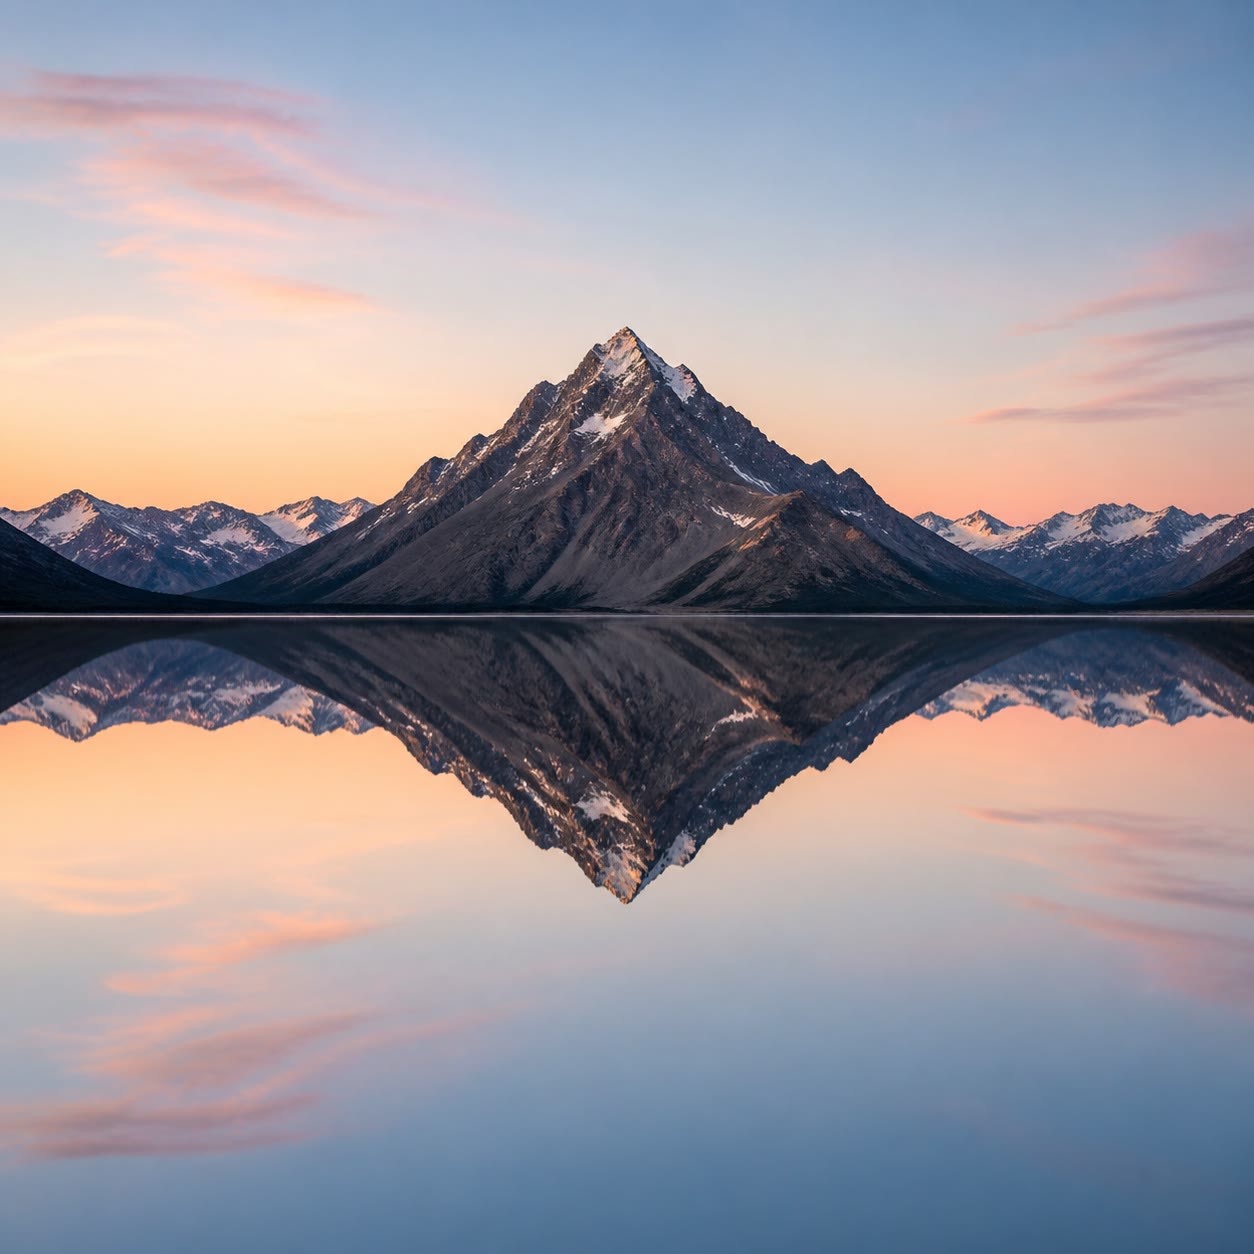
\includegraphics[width=0.45\linewidth]{images/book1/ai/g5-mirrors-lake.jpg}

{\small Um lago parado é um \omterm{def:g5:mirrors-reflection:reflection}{espelho} deitado: cada raio quica pela mesma regra, e a montanha aparece de novo, de cabeça para baixo e exata.}
\end{omfigure}

\section{A pessoa atrás do vidro}

\begin{proposition}[A regra da imagem]\label{prop:g5:mirrors-reflection:image}
Um \omterm{def:g5:mirrors-reflection:reflection}{espelho} plano mostra cada objeto como uma
\emph{imagem}\index{imagem} que fica \emph{atrás} do vidro,
exatamente tão atrás quanto o objeto está à frente, do mesmo tamanho,
ponto por ponto. Dê um passo para trás e a sua \omterm{prop:g5:mirrors-reflection:image}{imagem} também dá: o
mundo do \omterm{def:g5:mirrors-reflection:reflection}{espelho} é uma cópia fiel e dobrada do nosso.
\end{proposition}

\begin{omfigure}
\begin{tikzpicture}[scale=0.85]
  \draw[very thick] (5.5,0) -- (5.5,3.6);
  \fill[omThm] (2.5,2.6) circle (0.16);
  \draw[thick] (2.5,0.8) -- (2.5,2.4);
  \node[below, font=\small] at (2.5,0.5) {vela, \qty{1}{m} à frente};
  \fill[omThm, opacity=0.35] (8.5,2.6) circle (0.16);
  \draw[thick, omExo, dashed] (8.5,0.8) -- (8.5,2.4);
  \node[below, font=\small] at (8.5,0.5) {imagem, \qty{1}{m} atrás};
  \draw[omThm, thick] (2.5,2.6) -- (5.5,1.9);
  \draw[-Stealth, omThm, thick] (5.5,1.9) -- (3.4,0.35);
  \draw[omExo, dashed] (5.5,1.9) -- (8.5,2.6);
  \node[font=\small] at (3.2,0.15) {olho};
\end{tikzpicture}

{\small A regra da \omterm{prop:g5:mirrors-reflection:image}{imagem}: o olho recebe um raio quicado, mas o
prolonga em linha reta para trás --- até uma vela que parece estar
atrás do vidro, tão atrás quanto a vela verdadeira está à frente.}
\end{omfigure}

\begin{example}[Por que a imagem mora atrás]\label{ex:g5:mirrors-reflection:why}
O seu olho é uma alma simples: ele supõe que todo raio viajou em
linha reta. O raio quicado vem mesmo da vela, passando pelo \omterm{def:g5:mirrors-reflection:reflection}{espelho}
--- mas o olho o prolonga \emph{para trás, através do vidro}, até o
ponto de onde o raio parece ter partido. Todos os raios quicados
concordam com esse ponto de partida fantasma: os raios de uma vela,
uma vela fantasma bem nítida. Não há nada atrás da parede, claro ---
a \omterm{prop:g5:mirrors-reflection:image}{imagem} é a ilusão mais convincente da \omterm{def:g1:light-and-shadows:source}{luz}.
\end{example}

\begin{example}[O mundo trocado]\label{ex:g5:mirrors-reflection:swap}
Segure uma página escrita na frente do \omterm{def:g5:mirrors-reflection:reflection}{espelho}: as letras voltam
invertidas, com a esquerda e a direita trocadas. É por isso que a
palavra AMBULÂNCIA é pintada ao contrário na frente das ambulâncias:
os motoristas da frente, olhando pelos retrovisores, a veem voltar ao
normal --- e dão passagem. Dois \omterm{def:g5:mirrors-reflection:reflection}{espelhos} desfazem a troca: um quique
duplo inverte a inversão.
\end{example}

\section{Dobrar a estrada de propósito}

\begin{method}[Construir um periscópio]\label{met:g5:mirrors-reflection:periscope}
O olhador de esquinas prometido, entregue:
\begin{enumerate}
  \item pegue uma caixa alta e estreita; recorte uma janela perto do
        alto de uma das faces e outra perto da base da face oposta;
  \item fixe um espelhinho lá dentro atrás de cada janela, cada um
        inclinado em meio ângulo reto, com as duas inclinações
        paralelas entre si;
  \item aponte a janela de cima por cima do muro (ou depois da
        esquina) e olhe pela janela de baixo.
\end{enumerate}
A estrada da \omterm{def:g1:light-and-shadows:source}{luz} se dobra duas vezes: desce pela caixa entre os
\omterm{def:g5:mirrors-reflection:reflection}{espelhos} e depois sai até o seu olho. As tripulações de submarino
observam as ondas exatamente por um destes --- construído comprido e
à prova d'água.
\end{method}

\begin{omfigure}
\begin{tikzpicture}[scale=0.85]
  \draw[thick] (4.0,0) rectangle (5.6,4.4);
  \draw[very thick, omDef] (4.15,3.4) -- (5.45,4.25);
  \draw[very thick, omDef] (4.15,0.15) -- (5.45,1.0);
  \draw[-Stealth, omThm, very thick] (1.0,3.83) -- (4.8,3.83);
  \draw[-Stealth, omThm, very thick] (4.8,3.83) -- (4.8,0.58);
  \draw[-Stealth, omThm, very thick] (4.8,0.58) -- (8.4,0.58);
  \node[left, font=\small] at (0.9,3.83) {luz vinda da cena};
  \node[right, font=\small] at (8.5,0.58) {até o seu olho};
  \node[right, font=\small, omDef] at (5.7,4.0) {espelho inclinado};
  \node[right, font=\small, omDef] at (5.7,1.2) {espelho inclinado};
\end{tikzpicture}

{\small Dentro do periscópio: dois \omterm{def:g5:mirrors-reflection:reflection}{espelhos} inclinados e paralelos
dobram a estrada da \omterm{def:g1:light-and-shadows:source}{luz} duas vezes --- por cima do muro e até o seu
olho.}
\end{omfigure}

\begin{remark}[Colheres de casa de espelhos]\label{rem:g5:mirrors-reflection:curved}
Olhe para dentro da concha de uma colher polida: você fica pendurado
de cabeça para baixo. Vire a colher: você volta a ficar de pé, mas
esticado. Os \omterm{def:g5:mirrors-reflection:reflection}{espelhos} curvos continuam obedecendo à regra do quique
em cada ponto --- mas as ladeirinhas deles giram com a curvatura,
então os quiques ordenados se juntam ou se espalham, e as imagens
encolhem, crescem ou dão cambalhotas. Os \omterm{def:g5:mirrors-reflection:reflection}{espelhos} curvos também
concentram a \omterm{def:g1:light-and-shadows:source}{luz}: um prato curvo cheio de \omterm{def:g1:light-and-shadows:source}{luz} do Sol cozinha uma
panela --- lembre dos fogões solares do capítulo da \omterm{def:g5:everyday-energy:energy}{energia}. As leis
precisas deles pertencem a um ano mais adiante; a colher é a prévia
honesta.
\end{remark}

\section{Exercícios}

\begin{exercise}[$\star$]\label{exo:g5:mirrors-reflection:1}
Enuncie a regra do quique. O que faz um raio que chega perfeitamente
de frente?
\end{exercise}

\begin{exercise}[$\star$]\label{exo:g5:mirrors-reflection:2}
Uma parede branca reflete muita \omterm{def:g1:light-and-shadows:source}{luz}. Por que ela não mostra \omterm{prop:g5:mirrors-reflection:image}{imagem}
nenhuma, enquanto o \omterm{def:g5:mirrors-reflection:reflection}{espelho} polido mostra?
\end{exercise}

\begin{exercise}[$\star$]\label{exo:g5:mirrors-reflection:3}
Você está a \qty{2}{m} de um \omterm{def:g5:mirrors-reflection:reflection}{espelho} plano. Onde está a sua \omterm{prop:g5:mirrors-reflection:image}{imagem}, e
a que distância ela está de você?
\end{exercise}

\begin{exercise}[$\star$]\label{exo:g5:mirrors-reflection:4}
Você caminha na direção da sua \omterm{prop:g5:mirrors-reflection:image}{imagem} no \omterm{def:g5:mirrors-reflection:reflection}{espelho}, com passos lentos.
O que a \omterm{prop:g5:mirrors-reflection:image}{imagem} faz, e com que rapidez o vão entre vocês se fecha?
\end{exercise}

\begin{exercise}[$\star$]\label{exo:g5:mirrors-reflection:5}
Por que AMBULÂNCIA é pintado ao contrário na frente das ambulâncias?
Para quem a palavra fica legível, e através de quê?
\end{exercise}

\begin{exercise}[$\star$]\label{exo:g5:mirrors-reflection:6}
No periscópio, quantas vezes a estrada da \omterm{def:g1:light-and-shadows:source}{luz} se dobra, e o que cada
dobra faz? Com que inclinação ficam os \omterm{def:g5:mirrors-reflection:reflection}{espelhos}?
\end{exercise}

\begin{exercise}[$\star$]\label{exo:g5:mirrors-reflection:7}
Como um montanhista com um \omterm{def:g5:mirrors-reflection:reflection}{espelho} de bolso pode sinalizar para um
helicóptero distante? Quais duas ideias do capítulo estão em ação ---
diga a regra que mira o brilho e a reserva que o alimenta.
\end{exercise}

\begin{exercise}[$\star$]\label{exo:g5:mirrors-reflection:8}
A água parada espelha as montanhas; o \omterm{def:g2:air-around-us:wind}{vento} encrespa o lago e a
\omterm{prop:g5:mirrors-reflection:image}{imagem} se despedaça em cintilações. Explique os dois casos com o
\cref{ex:g5:mirrors-reflection:walls}.
\end{exercise}

\begin{exercise}[$\star\star$]\label{exo:g5:mirrors-reflection:9}
O olho ``prolonga os raios para trás''. Use isso para explicar por
que a sua \omterm{prop:g5:mirrors-reflection:image}{imagem} fica \emph{atrás} da parede em que o \omterm{def:g5:mirrors-reflection:reflection}{espelho} está
pendurado --- num lugar em que certamente não há ninguém. Com o que
todos os raios quicados vindos do seu nariz concordam?
\end{exercise}

\begin{exercise}[$\star\star$]\label{exo:g5:mirrors-reflection:10}
Uma loja quer que um cliente na porta enxergue o corredor depois de
uma esquina sem visão. Um único \omterm{def:g5:mirrors-reflection:reflection}{espelho} plano precisa ser montado no
encontro dos dois corredores. Como ele deve ser inclinado, e por que
a mesma montagem deixa o corredor enxergar a porta? (As estradas da
\omterm{def:g1:light-and-shadows:source}{luz} funcionam nos dois sentidos.)
\end{exercise}

\begin{exercise}[$\star\star$]\label{exo:g5:mirrors-reflection:11}
A escrita no \omterm{def:g5:mirrors-reflection:reflection}{espelho} volta invertida; um quique duplo ``inverte a
inversão''. Explique por que o periscópio do
\cref{met:g5:mirrors-reflection:periscope}, com os seus dois
\omterm{def:g5:mirrors-reflection:reflection}{espelhos}, mostra a cena no sentido certo e não espelhada.
\end{exercise}
